\documentclass[conference]{IEEEtran}
\IEEEoverridecommandlockouts
% The preceding line is only needed to identify funding in the first footnote. If that is unneeded, please comment it out.
\usepackage{cite}
\usepackage{amsmath,amssymb,amsfonts}
\usepackage{algorithmic}
\usepackage{graphicx}
\usepackage{textcomp}
\usepackage{xcolor}
\def\BibTeX{{\rm B\kern-.05em{\sc i\kern-.025em b}\kern-.08em
    T\kern-.1667em\lower.7ex\hbox{E}\kern-.125emX}}
\begin{document}

\title{MO443 - Assignment I}

\author{210404 -- Guilherme Vieira Leite}

\maketitle

\section{Introduction}

In this work we explore some variants of the dithering technique and their effect on images. The implemented variant of dithering is the error

\section{Dithering Methods}

The many implemented techniques differentiate by their mask and the way they are applied to the image.

\subsection{left2right}
\subsection{right2left}
\subsection{zigzag}

\section{Results}

\begin{figure}[htbp]
\centerline{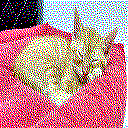
\includegraphics{figures/left2right/flo_color_juquinha.png}}
\caption{Example of a figure caption.}
\label{fig}
\end{figure}

\subsection{Error function}

\end{document}
